\documentclass[]{spie}  %>>> use for US letter paper
%\documentclass[a4paper]{spie}  %>>> use this instead for A4 paper
%\documentclass[nocompress]{spie}  %>>> to avoid compression of citations

\renewcommand{\baselinestretch}{1.0} % Change to 1.65 for double spacing
 
\usepackage{amsmath,amsfonts,amssymb}
\usepackage{graphicx}
\usepackage[colorlinks=true, allcolors=blue]{hyperref}

\title{Tunable Kernel-Nulling interferometry for direct exoplanet detection}

\author[a,*]{Vincent Foriel}
\author[a]{Frantz Martinache}
\author[a]{David Mary}
\affil[a]{Université Côte d’Azur, Observatoire de la Côte d’Azur Nice, CNRS, Laboratoire Lagrange, Nice, France}

\authorinfo{Further author information:\\Vincent Foriel - E-mail: vincent.foriel@oca.eu\\  Frantz Martinache - E-mail: frantz.martinache@oca.eu\\ Daid Mary - E-mail: david.mary@oca.eu}

% Option to view page numbers
\pagestyle{empty} % change to \pagestyle{plain} for page numbers   
\setcounter{page}{301} % Set start page numbering at e.g. 301
 
\begin{document}
\maketitle

\begin{abstract}

\end{abstract}

% Include a list of keywords after the abstract
\keywords{Interferometry, Exoplanet, Kernel-Nulling, VLTI, ASGARD}

\section{INTRODUCTION}
\label{sec:intro} % \label{} allows reference to this section

The direct detection of exoplanets is very challenging due to the high contrast between the stellar and planetary signals. Nulling interferometry offers a promising solution to this problem. This technique involves directing multiple telescopes at the target star to achieve destructive interference, effectively canceling out the star's light. Due to the angular separation between the star and its companion, the light from the latter reaches the telescopes with different phases, preventing complete destructive interference and allowing for potential constructive interference of the planetary light. However, such system is highly sensitive to phase aberations that limit their performances. Kernel-nulling is an attempt to partially overcome this issue by employing three or more [[[cite N telescope Laugier]]] telescopes to generate twin outputs that can be subtracted to eliminate low-order phase aberrations. This study aims to enhance the performance of such a system by reducing introducting phase aberation control techniques and statistical analysis to improve the detection of exoplanets.

\section{Architecture}

This study employs a 4-telescope Kernel-Nuller architecture, using integrated optical components. The interference is achieved through a series of 2x2 multimode interferometers (MMI) [[[cite paper presenting MMI]]]. There are two types of MMIs in this system. The first type, the nullers, perform constructive interference at the first output and destructive interference at the second output by placing the two signals in phase opposition (see Equation \ref{N} and Figure \ref{fig:nuller_and_recombiner}). The second type, referred to here as "recombiners," places the signals in phase quadrature (see Equation \ref{R} and Figure \ref{fig:nuller_and_recombiner}). These MMIs are separated by thermo-optic phase shifters that allow us to introduce phase shifts at various points in the system. The overall architecture is shown in Figure \ref{fig:kernel_nuller}.

The system has seven outputs: one bright output containing all four signals in phase synchronization, and six "dark" outputs containing combinations of signals in phase quadrature. Interestingly, these dark outputs occur in symmetric pairs (see Figure \ref{fig:phases}), meaning that a disturbance in one output will similarly affect the other output in the pair. This allows to cancel low-order phase aberations by subtracting the two dark outputs in each pair, creating a new observable called "kernels."

\begin{figure} [ht]
    \begin{center}
    \begin{tabular}{c}
    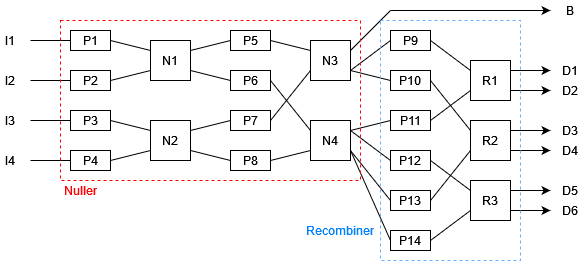
\includegraphics[height=6cm]{img/kernel_nuller.png}
    \end{tabular}
    \end{center}
    \caption[kernel_nuller] 
    { \label{fig:kernel_nuller} 
    Schematic of the tunable Kernel-Nuller architecture. P1-14 are the thermo-optic phase shifters. N1-4 are the four 2x2 Nuller MMIs, forming a 4x4 arrangement. R1-3 are the three recombiners that place the signals in phase quadrature. I1-4 are the input signals. B is the bright output and D1-6 are the dark outputs.}
\end{figure} 

\begin{figure} [ht]
    \begin{center}
    \begin{tabular}{c}
    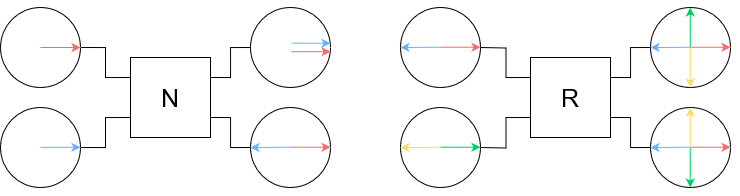
\includegraphics[height=3cm]{img/nuller_and_recombiner.png}
    \end{tabular}
    \end{center}
    \caption[nuller_and_recombiner] 
    { \label{fig:nuller_and_recombiner} 
    Schematic of the action of nuller (left) and recombiner (right) MMIs. The signals are represented by arrows in a complex polar plot showing the phase and amplitude of the signal. As we are insensitive to absolute phase, one signal (here the red one) is used as a reference.}
\end{figure}

\begin{equation}\label{N}
    N_n =
    \begin{pmatrix}
        1 & 1 \\
        1 & -1
    \end{pmatrix}
\end{equation}

\begin{equation}\label{R}
    R_n =
    \begin{pmatrix}
        e^{i\frac{pi}{4}} & e^{-i\frac{pi}{4}} \\
        e^{-i\frac{pi}{4}} & e^{i\frac{pi}{4}} \\
    \end{pmatrix}
\end{equation}

\begin{equation}\label{P}
    P_n = e^{i\theta_n}
\end{equation}

\section{Calibration}

Due to unavoidable manufacturing defects, the system will produce some phase aberrations that we aim to cancel using the active thermo-optic phase shifters. There are fourteen phase shifters in total, and we need to find the optimal values to place the signals in phase quadrature (see Figure \ref{fig:phases}) and optimize system performance. To achieve this, we use a genetic algorithm to explore the parameter space and find these optimal values.

\begin{figure} [ht]
    \begin{center}
    \begin{tabular}{c}
    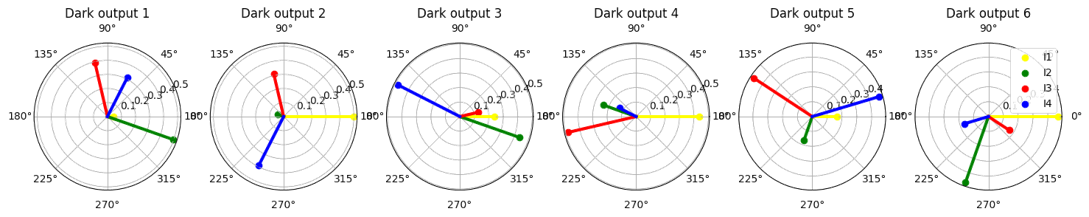
\includegraphics[height=2.5cm]{img/perturbed_phase.png}\\
    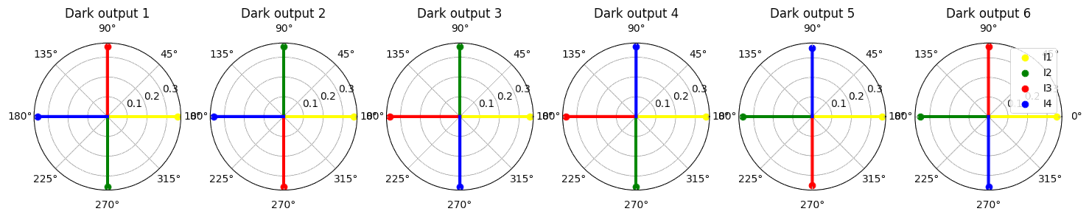
\includegraphics[height=2.5cm]{img/calibrated_phase.png}
    \end{tabular}
    \end{center}
    \caption[phases] 
    { \label{fig:phases} 
    RPolar representation of the complex amplitudes obtained at the dark outputs. Each output is a combination of signals from the 4 telescopes, ideally separated by 90°. The first line is what we get without calibrating the system. We observe that phase perturbations of the order of $\lambda / 10$ cause significant performance degradation. However, the convergence algorithm effectively corrects these perturbations, restoring the signals to phase quadrature.}
\end{figure}

During the calibration phase, we consider a single star without phase perturbation at the input. In this case, all the light flux should be directed to the bright output, and all kernels should be perfectly null. We use two metrics to evaluate system performance:

\begin{equation}
    M_B = |B|^2
\end{equation}

\begin{equation}
    M_K = \Big||D_1|^2 - |D_2|^2\Big|+\Big||D_3|^2 - |D_4|^2\Big|+\Big||D_5|^2 - |D_6|^2\Big|
\end{equation}

Each phase shifter is associated with a performance metric. Phase shifters $P_1$ to $P_5$ and $P_7$ (see Figure \ref{fig:kernel_nuller}) are associated with the $M_B$ metric as they contribute to redirecting the flux to the bright output. The remaining phase shifters are associated with the $M_K$ metric. The goal of the genetic algorithm is to maximize $M_B$ and minimize $M_K$.

Iteratively, the algorithm adjusts the value of a phase shifter and observes the impact on the associated metric. If the metric improves, the change is kept; otherwise, it is discarded. This process is repeated for each phase shifter in a loop, reducing the modification step size each time. The algorithm stops when the modification step size is below a certain threshold, corresponding to the precision with which we can adjust the phase shifters.

\section{Performances}

The calibration corrects phase errors caused by manufacturing defects but does not address phase errors occurring upstream, such as those induced by the atmosphere. For each observation, we obtain an intensity value for each kernel that is not exactly as expected but distributed around this value, with a dispersion that directly dependent on the phase perturbations (see Figure \ref{fig:distrib}).

\begin{figure} [ht]
    \begin{center}
    \begin{tabular}{c}
    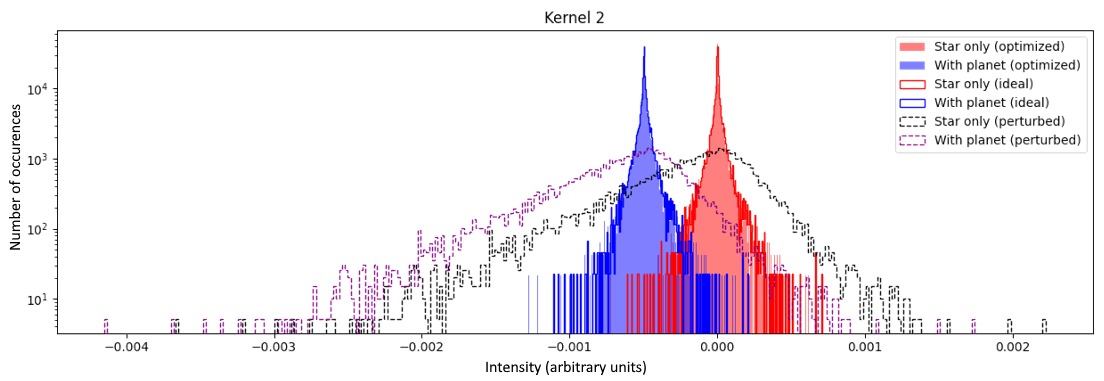
\includegraphics[height=5cm]{img/distrib.png}
    \end{tabular}
    \end{center}
    \caption[distrib] 
    { \label{fig:distrib} 
    Intensity distributions obtained on a kernel for both hypotheses (with and without a planet). We see that distributions obtained after the calibration algorithm has converged closely match the distributions expected with an ideal component. To clearly see the distribution shift due to the presence of a planet, the contrast has been set to $10^{-3}$, and the RMS phase perturbation is set to $\lambda / 100$ ($16.5$nm).}
\end{figure}

We can use these distributions to estimate the presence of a planet. If a planet is present, the intensity distribution will shift compared to the expected distribution without a planet. Statistical tests can then be used to evaluate the presence of a planet. So far, only simple tests have been conducted (see Figure \ref{fig:ROC}), reducing the distribution to a single intensity value using the mean, median, and argmax of the obtained distribution and comparing this intensity to a threshold value.

\begin{figure} [ht]
    \begin{center}
    \begin{tabular}{c}
    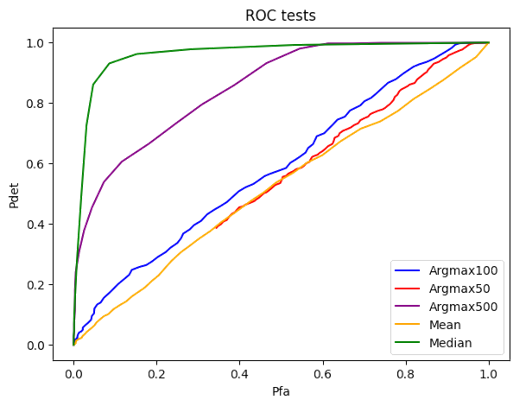
\includegraphics[height=5cm]{img/ROC.png}
    \end{tabular}
    \end{center}
    \caption[ROC] 
    { \label{fig:ROC} 
    This plot shows the detection performance (Pdet) as a function of the probability of false alarm (Pfa) for different methods. The methods used here consist of reducing the distribution to a single value using the median, mean, and argmax operations and comparing this value to a threshold. The higher the threshold, the more the null hypothesis is favored. The lower the threshold, the more false alarms we encounter.}
\end{figure}

For a series of observations with the same parallactic angle, simple statistical tests like those studied here are theoretically sufficient to detect planets with a contrast of $10^{-5}$ in the presence of phase perturbations of the order of $\lambda / 100$ in 90\% of cases with a 1\% probability of false alarm. While very encouraging, these results must be confirmed by laboratory tests.

\section{Position caracterization}

The next step is to determine the position of the detected planet. To do this, we perform a series of observations at various parallactic angles. Using the transmission maps of the different kernels (see Figure \ref{fig:transmission_map}), we can determine the expected signal modulation for a planet at a given location. By fitting this function to the obtained data, we can determine the planet's position (Figure \ref{fig:fit}).

\begin{figure} [ht]
    \begin{center}
    \begin{tabular}{c}
    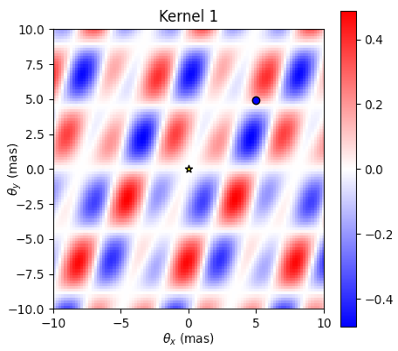
\includegraphics[height=5cm]{img/transmission_map.png}
    \end{tabular}
    \end{center}
    \caption[transmission_map] 
    { \label{fig:transmission_map} 
    Depending on the telescope positions, certain angles will result in phase differences that either constructively or destructively interfere. This phenomenon leads to a transmission map, different for each kernel. As kernels are built using the difference in intensity of two dark outputs, this transmission map can go negative. If a planet is positioned in a red zone, the obtained distribution (Figure \ref{fig:distrib}) will shift towards positive values, and if it is in a blue zone, it will shift towards negative values.}
\end{figure}

\begin{figure} [ht]
    \begin{center}
    \begin{tabular}{c}
    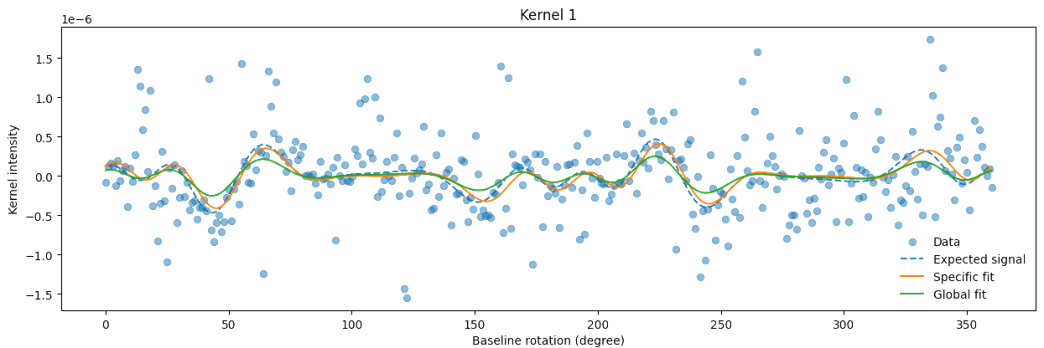
\includegraphics[height=5cm]{img/fit.png}
    \end{tabular}
    \end{center}
    \caption[fit] 
    {\label{fig:fit} 
    To determine the position of the planet, we fit the signal modulation function to the obtained data. This fitting process is conducted for each kernel individually, referred as the "specific fit". After performing the specific fits, we average the resulting positions to derive a new position estimate. We then plot the modulation for this averaged position, referred to as the "global fit".}
\end{figure}

The modulation function's complexity makes it difficult for the fitting algorithm to converge unless it is initially given an approximate but close position and contrast to the expected true parameters. Unfortunately, we lack this information. One approach is to perform the fit by using each point in the sky as an initial parameter and identifying when the fit properly converges using a correlation indicator.

An alternative solution is to generate a sky map highlighting the regions that could potentially have contributed to the observed data. This method involves weighting each rotated transmission map by the data obtained for that specific parallactic angle, then summing all the weighted maps (Figure \ref{fig:contribution_zone}).

\begin{figure} [ht]
    \begin{center}
    \begin{tabular}{c}
    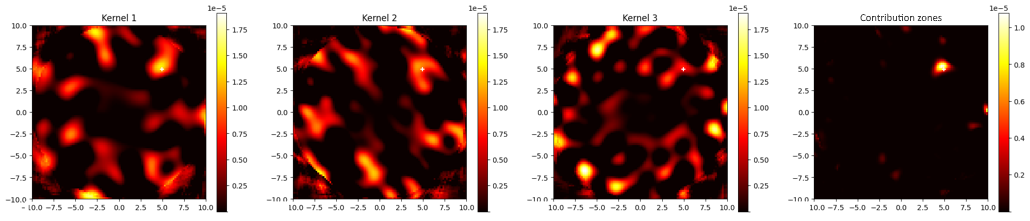
\includegraphics[height=3.5cm]{img/contribution_zone.png}
    \end{tabular}
    \end{center}
    \caption[contribution_zone] 
    {\label{fig:contribution_zone} 
    Each of the first three plots represents the sum of the contribution maps oriented at a specific parallactic angle, weighted by the data obtained for that angle. The final plot represents the product of the first three plots.}
\end{figure}

\section{Discussion \& Prospects}

Simulation results are highly encouraging, showing detection performance comparable to current techniques and indicating the potential for even greater contrast by leveraging angular diversity. However, these results must be validated through laboratory tests.

Several factors could reduce these performances, such as amplitude aberrations, the chromatic nature of light, or the presence of multiple objects around the star. Adding these constraints to the simulation model and conducting an in-depth study on possible statistical tests will help to better define the actual limitations of such a system.

\acknowledgments

Thanks to Romain Laugier for his wise advice, to Nick Cvetojevic for his introduction to the topic of photonics and to Margaux Abello for her presentation recommendations. This thesis is made possible by the PHOTONICS project of the PEPR ORIGINS and Thales Alenia Space



\begin{thebibliography}{60}

    \bibitem{Martinache et al. 2018}  Martinache, Frantz, et Michael J. Ireland. "Kernel-Nulling for a Robust Direct Interferometric Detection of Extrasolar Planets". {\it Astronomy \& Astrophysics} \textbf{619} (2018): A87. https://doi.org/10.1051/0004-6361/201832847.
    
    
    \bibitem{Cvetojevic et al. 2022} Cvetojevic, N. et al. 3-beam self-calibrated Kernel nulling photonic interferometer (2022). Preprint at http://arxiv.org/abs/2206.04977.
    
\end{thebibliography}

% References
% \bibliography{report} % bibliography data in report.bib
% \bibliographystyle{spiebib} % makes bibtex use spiebib.bst

\end{document}